
\documentclass{article}

\usepackage{titlesec}
\newcommand{\sectionbreak}{\clearpage}

\usepackage{fancyhdr}
\pagestyle{fancy}
\lhead{Emanuel Casiano-Diaz}
\rhead{CSYS300: PoCS - Homework 05 - 10/05/2018}
\renewcommand{\headrulewidth}{0.4pt}
\renewcommand{\footrulewidth}{0.4pt}

\usepackage{amsmath}
\usepackage{amssymb}
\usepackage{bm}
\usepackage{pdfpages}

\usepackage{enumerate}% http://ctan.org/pkg/enumerate

\usepackage{hyperref}
\hypersetup{
    colorlinks=true,
    linkcolor=blue,
    filecolor=magenta,      
    urlcolor=cyan,
}

\usepackage{booktabs,float,siunitx}
%\usepackage[demo]{graphicx} % omit 'demo' option in real document

\begin{document}

\section{Exercise 1: Generalized entropy and diversity}

Strategy: Equate the corresponding information measure of text $T$ to that of text $T'$ and solve for the diversity, $D$. The probabilities will be given by $p_i = \frac{1}{D}$.

\subsection{a) Simpson Concentration}
\begin{align}
S[T] &= S[T'] \\
&= \sum_{j=1}^{D} p_j^2 \\
&= \sum_{j=1}^{D} (\frac{1}{D})^2 \\
&= (D) (\frac{1}{D^2}) \\
S[T] &= D^{-1} = \sum_{i=1}^{n} p_i^2 \\
\implies D &= \frac{1}{\sum_{i=1}^{n} p_i^2}
\end{align}

\subsection{b) Gini Index}
\begin{align}
G[T] &= G[T'] \\
&= 1 - \sum_{j=1}^{D} p_j^2 \\
G[T ] &= 1 - D^{-1} = 1 - \sum_{i=1}^{n} p_i^2 \\
\implies D &= \frac{1}{\sum_{i=1}^{n} p_i^2} 
\end{align}

The Simpson Concentration and Gini Concentration have the same diversity! 

\subsection{c) Shannon Entropy}
\begin{align}
H[T] &= H[T'] \\
&= - \sum_{j=1}^D p_j \ln p_j \\
&= - (D) (\frac{1}{D}) \ln (\frac{1}{D}) \\
&= -\ln(\frac{1}{D}) \\
H[T] &= \ln D = - \sum_{i=1}^{n} p_i \ln p_i \\
\implies D &= e^{-\sum p_i \ln p_i}
\end{align}

Note: In the line above, the lower and upper limits of the summation have been left out for esthetic reasons.

\subsection{d) Renyi Entropi}
\begin{align}
H_{q}^{(R)}[T] = H_{q}^{(R)}[T'] \\
&= \frac{1}{q-1} [-\ln \sum_{j=1}^D p_j^q] \\
&= \frac{1}{1-q}\ln [(D)(\frac{1}{D})^q] \\
&= \frac{1}{1-q} \ln [D^{1-q}] \\
H_q^{(R)} &= \ln D = \frac{1}{1-q} \ln \sum_{i=1}^{n} p_i^q \\
\implies D &= [\sum_{i=1}^n p_i^q]^{\frac{1}{1-q}}
\end{align}
\subsection{e) Generalized Tsallis Entropy}

\begin{align}
H_q^{(Ts)} [T] &= H_q^{(Ts)} [T'] \\
&= \frac{1}{q-1} - \frac{1}{q-1} [\ln \sum_{j=1}^D p_j^q]  \\
H_q^{(Ts)} [T] &= \frac{1}{q-1} + \ln D = \frac{1}{q-1} - \frac{1}{q-1} [\ln \sum_{i=1}^D p_i^q] \\
\implies \ln D &= - \frac{1}{q-1} [\ln \sum_{i=1}^D p_i^q] \\
\implies D &=  [\sum_{i=1}^n p_i^q]^{\frac{1}{1-q}}
\end{align}

The Renyi Entropy and Generalized Tsallis Entropy have the same diversity!

\subsection{f) The limiting case of $q \to 1$}

Here it will be shown that as $q\to1$, the diversity of the Renyi and Generalized Tsallis Entropy becomes the diversity of the Shannon Entropy. For simplicity (hopefully), the limit will be evaluated for $\ln D$ instead, then exponentiated at the end.

\begin{align}
\lim_{q\to1} \ln D = \lim_{q \to 1} \frac{\ln[\sum_{i=1}^n p_i^q]}{1-q} = \frac{0}{0}
\end{align}

Recall that the probabilities are normalized. In other words, $\sum_{i} = p_i = 1$ and $\ln{1} = 0$. This is the reason why the indeterminate form $\frac{0}{0}$ is obtained. Applying L'Hopital's Rule once will get rid of this issue:

\begin{align}
\lim_{q\to1} \ln D &=  -\lim_{q\to1} \frac{d}{dq} [\sum_i p_i^q] ; \text{ via L'Hopital} \\
\end{align}
\\
Now, there's three rules that will be convenient to recall: \\
\\
1. Differential operators can be interchanged with summations \\
2. $\frac{d}{dx} \ln f(x) = \frac{f'(x)}{f(x)}$ \\
3. $\frac{d}{dx} a^x = a^x \ln a$, where $a>0$ and $a\neq1$ \\

Thus, applying these to the right hand side (RHS) of the above equation, the limit becomes:

\begin{align}
\lim_{q\to1} \ln D &= -\lim_{q\to1} \ln[\frac{\sum_i p_i^q \ln p_i}{\sum_i p_i^q}]
 \end{align}

Applying the normalization condition to the denominator in the RHS:

\begin{align}
\lim_{q\to1} \ln D &= -\lim_{q\to1} \ln [\sum_i p_i^q \ln p_i] = -\ln [\sum_i p_i \ln p_i] \\
\implies \lim_{q\to1} D &= exp[-\ln \sum_i p_i \ln p_i]
\end{align}

$\therefore$ In the limit $q\to1$, the Diversity of the Renyi and Generalized Tsallis Entropies becomes the Shannon Entropy Diversity!

\section{Exercise 2}

Want: The set of probabilities $p_i$ that minimize $\Psi$. Thus, need to solve the following equation for $p_i$:

\begin{align}
\frac{d\Psi}{dp_i} &= \frac{dF}{dp_i} + \lambda \frac{dG}{dp_i} = 0
\end{align}

NOTE: The derivatives are rather extensive to type in LaTeX in excruciating detail. As such, only the key ideas behind it will be discussed here. To see my full derivation, please follow this link: \url{} 

\section{Exercise 3}
\subsection{a)}
\subsection{b)}
\section{Exercise 4}


\end{document}

\begin{figure}[h!]
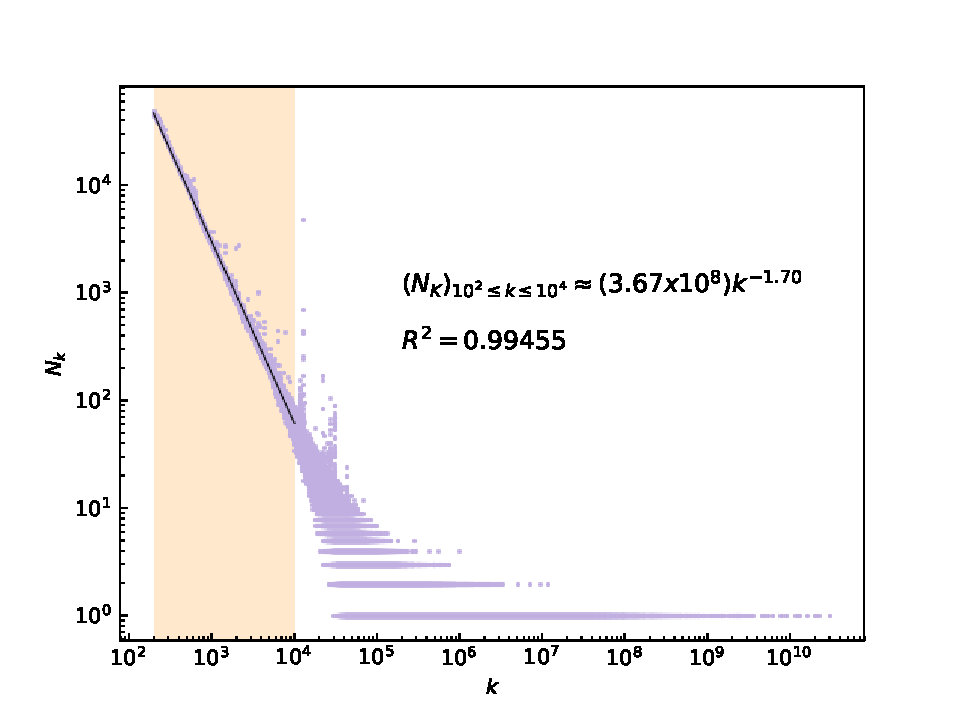
\includegraphics[width=\linewidth]{Q06/wordFrequencyLog.pdf}
\caption{Frequency $k$ that groups of $N_k$ words are repeated in a Google data set plotted in a base 10, log-log scale. The orange region denotes where power-law scaling holds (via "eye-balling"). By doing a linear regression on the sets $\log_{10} N_k$  ($y-$values) and $\log_{10} k$ ($x-$values) only inside the orange region, the prefactor and scaling exponent have been estimated to be $A \approx 3.67 x 10^{8}$ and $p \approx -1.70$, respectively.}
\label{fig:envelope}
\end{figure}